% Digital Logic Report Template
% Created: 2020-01-10, John Miller

%==========================================================
%=========== Document Setup  ==============================

% Formatting defined by class file
\documentclass[11pt]{article}

% ---- Document formatting ----
\usepackage[margin=1in]{geometry}	% Narrower margins
\usepackage{booktabs}				% Nice formatting of tables
\usepackage{graphicx}				% Ability to include graphics

%\setlength\parindent{0pt}	% Do not indent first line of paragraphs 
\usepackage[parfill]{parskip}		% Line space b/w paragraphs
%	parfill option prevents last line of pgrph from being fully justified

% Parskip package adds too much space around titles, fix with this
\RequirePackage{titlesec}
\titlespacing\section{0pt}{8pt plus 4pt minus 2pt}{3pt plus 2pt minus 2pt}
\titlespacing\subsection{0pt}{4pt plus 4pt minus 2pt}{-2pt plus 2pt minus 2pt}
\titlespacing\subsubsection{0pt}{2pt plus 4pt minus 2pt}{-6pt plus 2pt minus 2pt}

% ---- Hyperlinks ----
\usepackage[colorlinks=true,urlcolor=blue]{hyperref}	% For URL's. Automatically links internal references.

% ---- Code listings ----
\usepackage{listings} 					% Nice code layout and inclusion
\usepackage[usenames,dvipsnames]{xcolor}	% Colors (needs to be defined before using colors)

% Define custom colors for listings
\definecolor{listinggray}{gray}{0.98}		% Listings background color
\definecolor{rulegray}{gray}{0.7}			% Listings rule/frame color

% Style for Verilog
\lstdefinestyle{Verilog}{
	language=Verilog,					% Verilog
	backgroundcolor=\color{listinggray},	% light gray background
	rulecolor=\color{blue}, 			% blue frame lines
	frame=tb,							% lines above & below
	linewidth=\columnwidth, 			% set line width
	basicstyle=\small\ttfamily,	% basic font style that is used for the code	
	breaklines=true, 					% allow breaking across columns/pages
	tabsize=3,							% set tab size
	commentstyle=\color{gray},	% comments in italic 
	stringstyle=\upshape,				% strings are printed in normal font
	showspaces=false,					% don't underscore spaces
}

% How to use: \Verilog[listing_options]{file}
\newcommand{\Verilog}[2][]{%
	\lstinputlisting[style=Verilog,#1]{#2}
}




%======================================================
%=========== Body  ====================================
\begin{document}

\title{ELC 2137 Lab 4: Subtractor}
\author{Trevor Jackson, Carlos Hernandez, and Makenna Meyers}

\maketitle


\section*{Summary}

This lab was an extension of the previous adders lab, in which a family of logic chips was used to design logic circuits. The full adder and two-bit adder were reproduced, and we were charged with determining what needed to be added to the two-bit adder circuit to convert it to a subtractor circuit. As shown in Figure \ref{fig:Subtractor_Schematic}, three XOR gates were needed for the conversion from a two-bit adder circuit to a subtractor circuit. Like the previous circuits, the subtractor circuit was built and tested. The constructed circuit can be found in Figure \ref{fig:Subtractor_Circuit}, and the expected and actual results can be found in Figure \ref{fig:Circuit_Demonstration}.

\section*{Q\&A}

\begin{enumerate}
	\item Why did we use two full adders instead of a half adder and a full adder?

  The half adder only has two inputs whereas the full adder has three. There are six possible inputs for the subtractor circuit (A1, B1, A2, B2, Cin, and M), so using two full adders simplifies the circuits. The subtractor circuit was built from a two bit adder circuit, which only has five inputs. An additional input location was necessary to complete the subtractor circuit, as M was added as an input. As shown in Figure \ref{fig:Subtractor_Schematic}, M takes the place of Cin, so only five inputs are used. It is possible, however, to build a subtractor circuit with Cin and M as separate inputs, and it would be easier to do so with two full adders instead of a half hald and a full adder. 
	
	\item How many input combinations would it take to exhaustively test the adder/subtractor?

With the M and Cin as separate switches/inputs, there are $2^6$ possibilities and with M and Cin as one switch there are $2^5$ possiblities.

	\item Why were the combinations given in the truth table chosen?

The combinations in the truth table were given because they represent all the possible outputs from the circuit. Even though the full truth table has eight different inputs, there are only six unique outputs from the circuit because some inputs produce identical outputs.

    \item Do the results from your adder/subtractor math what you would expect from theory? Explain any discrepancies.
    
Initially, the results from the circuit provided an inverted value for the borrow bit due to the overflow of the operation. However, this issue was rectified via inverting the MSB when using the subtractor operation. Inverting the MSB required an additional exclusive-or gate to be added to the end of the circuit, which then allowed the theoretical and experimental results to coincide.
   
\end{enumerate}

\section*{Results}

The connections in some of the switches on the blue box were problematic, so we had to incorporate additional wires and switches to let the adder/subtractor circuit function properly. We also used two additional XOR gates instead of one for the M connections.

\clearpage
	
\begin{figure}\centering
	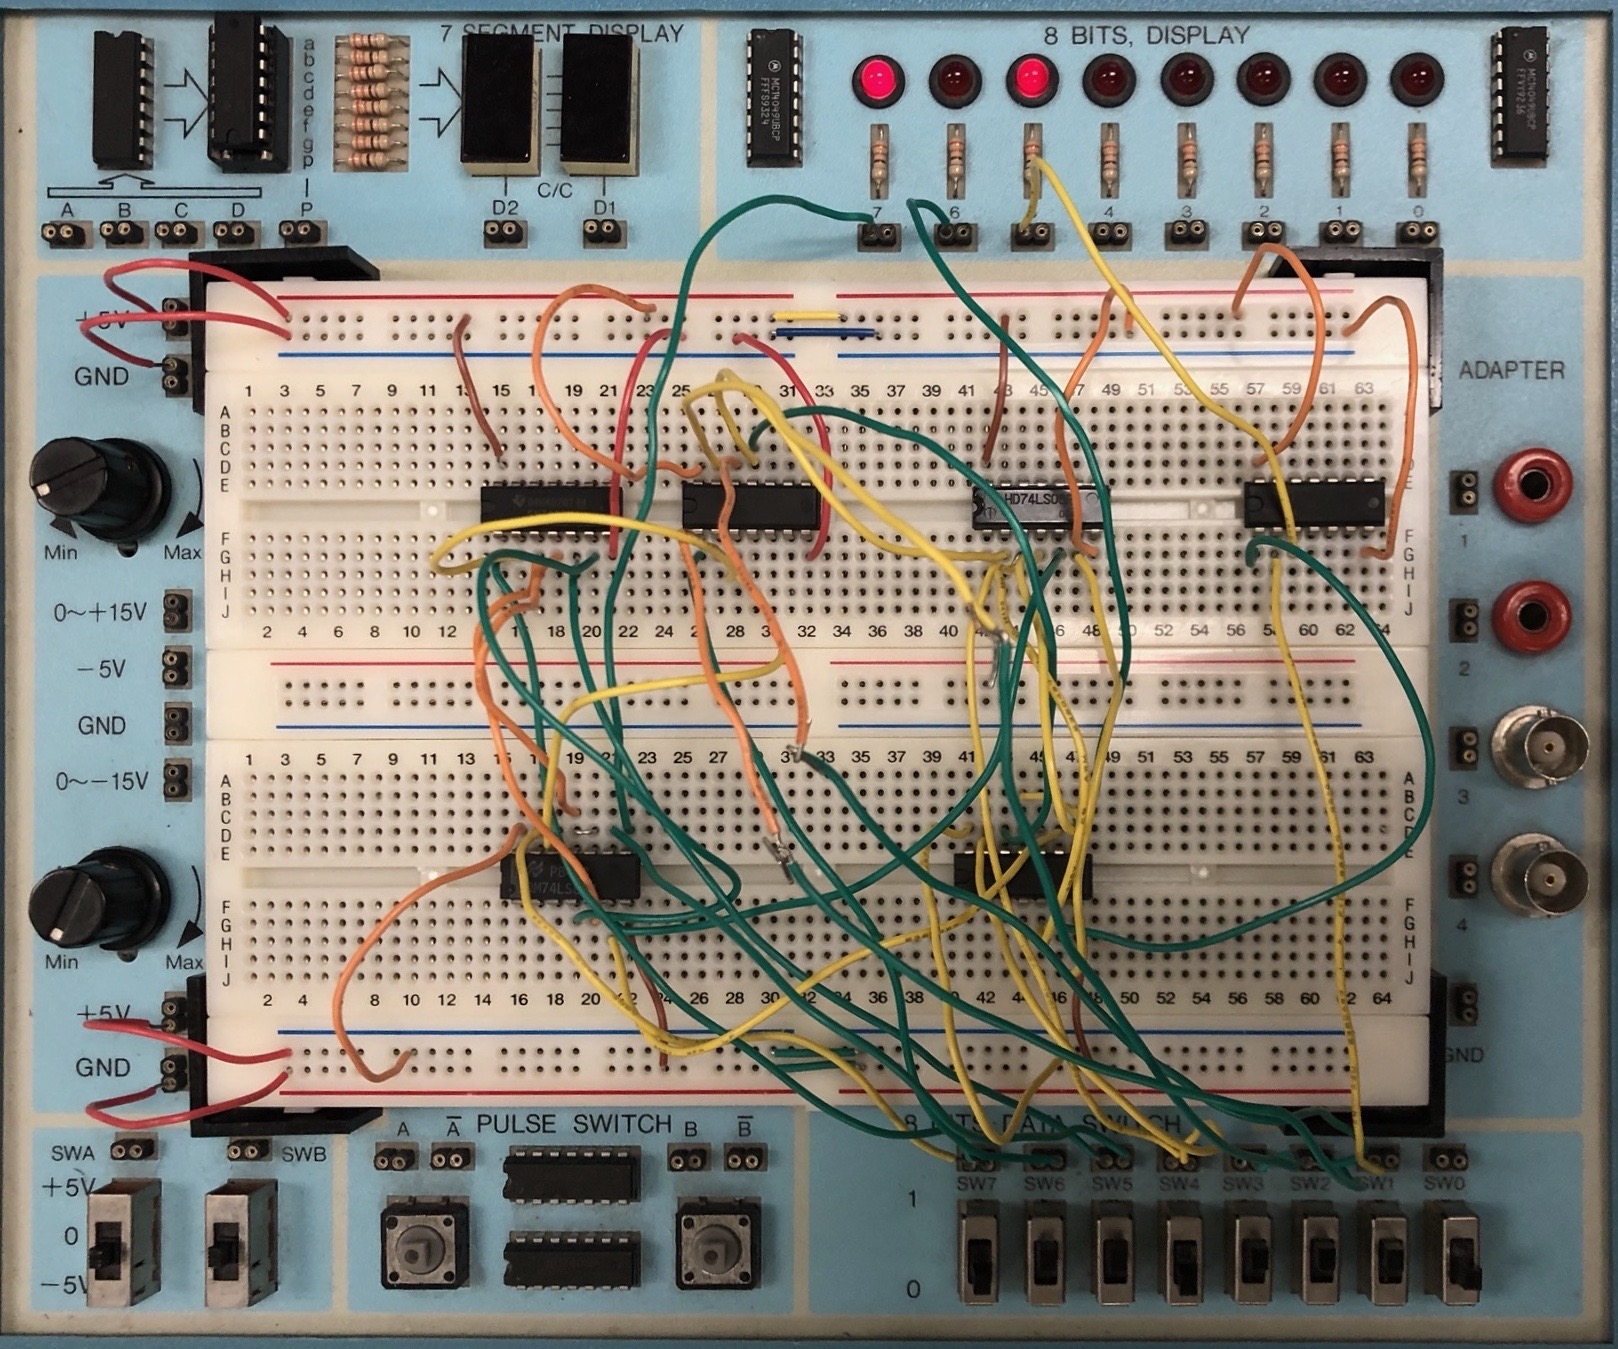
\includegraphics[width=0.8\textwidth,trim=0cm 0cm 0cm 0cm,clip]{Assembled_Subtractor}
	\caption{Assembled Subtractor Circuit}
	\label{fig:Subtractor_Circuit}	
\end{figure}

\begin{figure}\centering
	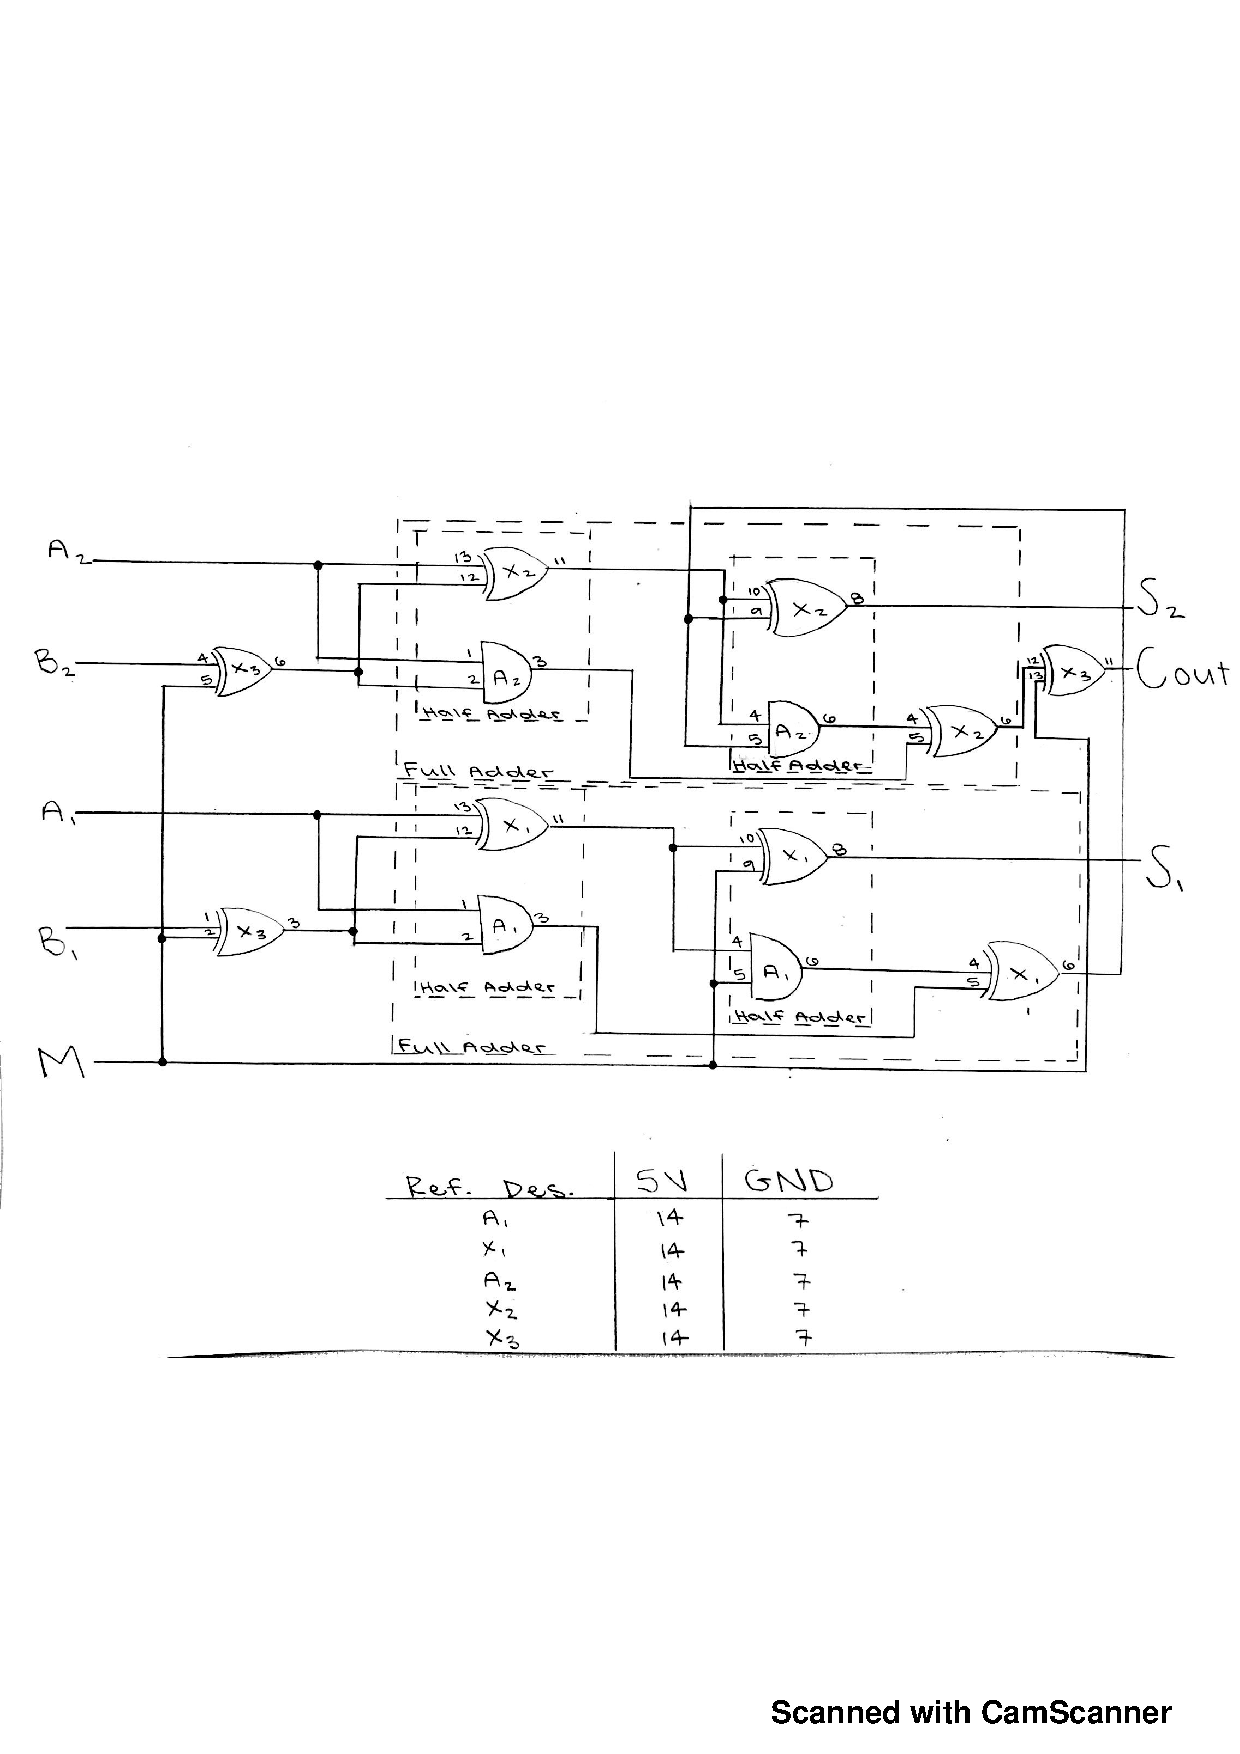
\includegraphics[width=0.8\textwidth,trim=0.3cm 6.8559cm 0cm 8cm,clip]{Two_Bit_Adder_and_Subtractor_Schematic}
	\caption{Two Bit Adder/Subtractor Schematic}
	\label{fig:Subtractor_Schematic}	
\end{figure}

\begin{figure}\centering
	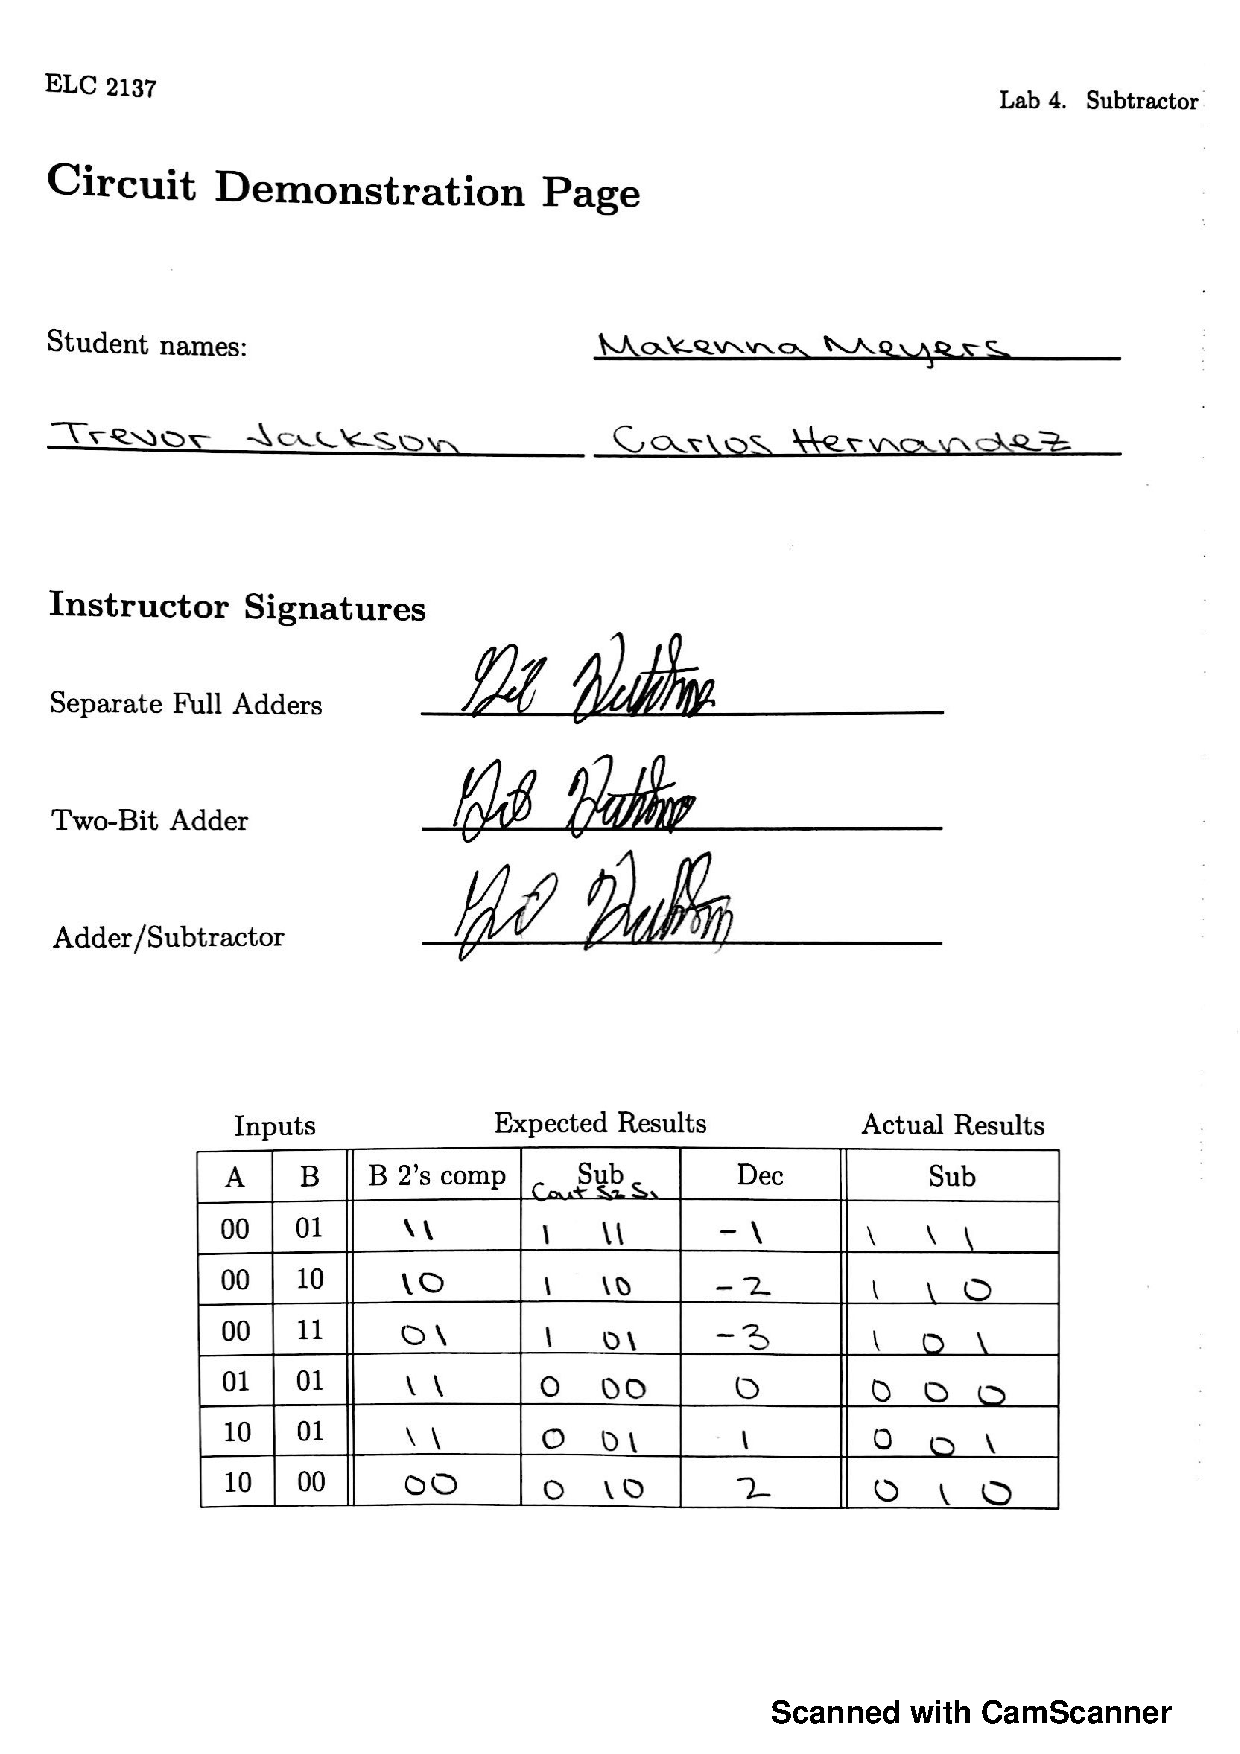
\includegraphics[width=0.8\textwidth,trim=0cm 3cm 0cm 0cm,clip]{Lab4_Circuit_Demonstration_Page} 
	\caption{In-Class Circuit Demonstration}
	\label{fig:Circuit_Demonstration}
\end{figure}	

\end{document}
